\tp{Mesure de l'indice d'un prisme}

\vressort{3}

\section{Visualisation du spectre de la lampe � vapeur de mercure}



\begin{itemize}
\item Placez le prisme sur la plate-forme de fa�on � ce que :
 son ar�te soit proche de centre
 la lumi�re incidente soit quasiment rasante ($i$ grand)

\item Recherchez et observez � la lunette le spectre obtenu (se rappeler pour cela dans quelle sens a lieu la d�viation de la lumi�re)

\item Observez quelles sont les radiations les plus d�vi�es

\item Choisissez une longueur d'onde. Observer l'existence d'un
  minimum de d�viation.


Rappel : il s'agit d'une d�viation minimum en fonction de l'angle d'incidence. Il faut donc ici modifier l'angle d'incidence en faisant tourner la plate-forme ; suivre le  spectre � la lunette : $D$ diminue puis r�augmente.


\end{itemize}


\vressort{3}


\section{Mesure de l'angle de d�viation minimal}

\begin{center}
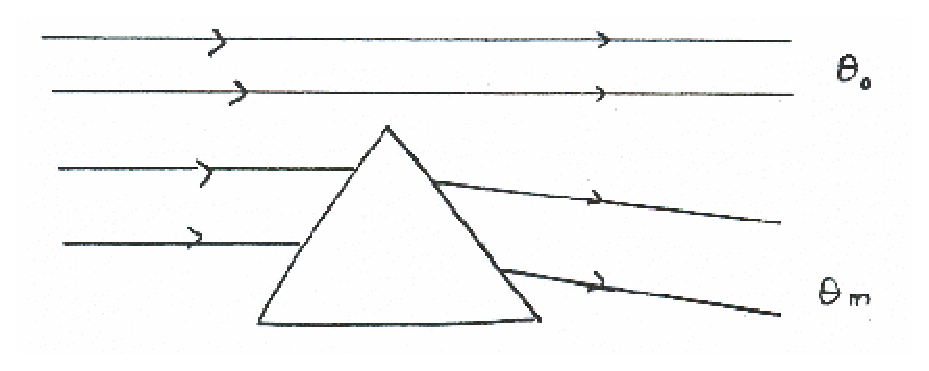
\includegraphics{opt/tp_prisme_indice/prisme_dev_mini.gif.eps}
\end{center}


\begin{itemize}

\item Pointez la direction incidente (mesure $\theta_0$).

\vressort{1}

\item Pointez pour la raie jaune-vert intense du mercure le faisceau
  d�vi� au minimum de d�viation (mesure $\theta_m$).

\vressort{1}

\item D�duisez $D_m = \theta_m - \theta_0$.

\end{itemize}

\vressort{2}

Pour effectuer le point�,


\begin{itemize}
\item Faites le d'abord approximativement.

\vressort{1}

\item Fixez la plate-forme et la lunette.

\vressort{1}

\item Agissez sur la vis fine d'orientation de la plate-forme pour se
  placer au minimum de d�viation.

\vressort{1}

\item Agissez sur la vis fine de d�placement fin de la lunette pour
  pointer la raie.

\vressort{1}

\item La longueur d'onde de la raie jaune-vert du mercure est de
  $0,5460~\mu m$.

\end{itemize}



\vressort{3}


\section{Conclusion}
D�duisez l'indice du prisme pour cette longueur d'onde.

